% Created 2025-06-17 Tue 22:20
% Intended LaTeX compiler: pdflatex
\documentclass[smaller, aspectratio=169]{beamer}\usepackage{listings}
\usepackage{color}
\usepackage{amsmath}
\usepackage{array}
\usepackage[T1]{fontenc}
\usepackage{natbib}
\lstset{
keywordstyle=\color{blue},
commentstyle=\color{red},stringstyle=\color[rgb]{0,.5,0},
literate={~}{$\sim$}{1},
basicstyle=\ttfamily\small,
columns=fullflexible,
breaklines=true,
breakatwhitespace=false,
numbers=left,
numberstyle=\ttfamily\tiny\color{gray},
stepnumber=1,
numbersep=10pt,
backgroundcolor=\color{white},
tabsize=4,
keepspaces=true,
showspaces=false,
showstringspaces=false,
xleftmargin=.23in,
frame=single,
basewidth={0.5em,0.4em},
}
\usepackage{natbib, dsfont, pgfpages, tikz,amssymb, amsmath,xcolor}
\bibliographystyle{abbrvnat}
\setbeamertemplate{footline}[frame number]
\beamertemplatenavigationsymbolsempty
\usepackage{appendixnumberbeamer}
\setbeamercolor{gray}{bg=white!90!black}
\setbeamertemplate{itemize items}{$\circ$}
\renewcommand{\thefootnote}{\fnsymbol{footnote}}
\RequirePackage{fancyvrb}
\DefineVerbatimEnvironment{verbatim}{Verbatim}{fontsize=\footnotesize}
\definecolor{bblue}{rgb}{0.2,0.2,0.7}
\newcommand{\E}{{\ensuremath{\mathop{{\mathbb{E}}}}}}
\newcommand{\R}{\mathbb{R}}
\newcommand{\N}{\mathbb{N}}
\newcommand{\blank}{\makebox[1ex]{\textbf{$\cdot$}}}
\newcommand\independent{\protect\mathpalette{\protect\independenT}{\perp}}
\def\independenT#1#2{\mathrel{\rlap{$#1#2$}\mkern2mu{#1#2}}}
\renewcommand{\phi}{\varphi}
\renewcommand{\epsilon}{\varepsilon}
\newcommand*\diff{\mathop{}\!\mathrm{d}}
\newcommand{\weakly}{\rightsquigarrow}
\newcommand\smallO{\textit{o}}
\newcommand\bigO{\textit{O}}
\newcommand{\midd}{\; \middle|\;}
\newcommand{\1}{\mathds{1}}
\usepackage{ifthen} %% Empirical process with default argument
\newcommand{\G}[2][n]{{\ensuremath{\mathbb{G}_{#1}}{\left[#2\right]}}}
\DeclareMathOperator*{\argmin}{\arg\!\min}
\DeclareMathOperator*{\argmax}{\arg\!\max}
\newcommand{\V}{\mathrm{Var}} % variance
\newcommand{\eqd}{\stackrel{d}{=}} % equality in distribution
\newcommand{\arrow}[1]{\xrightarrow{\; {#1} \;}}
\newcommand{\arrowP}{\xrightarrow{\; P \;}} % convergence in probability
\newcommand{\KL}{\ensuremath{D_{\mathrm{KL}}}}
\newcommand{\leb}{\lambda} % the Lebesgue measure
\DeclareMathOperator{\TT}{\Psi} % target parameter
\newcommand{\empmeas}{\ensuremath{\mathbb{P}_n}} % empirical measure

\renewcommand*\familydefault{\sfdefault}
\itemsep2pt
\usepackage[utf8]{inputenc}
\usepackage[T1]{fontenc}
\usepackage{graphicx}
\usepackage{longtable}
\usepackage{wrapfig}
\usepackage{rotating}
\usepackage[normalem]{ulem}
\usepackage{amsmath}
\usepackage{amssymb}
\usepackage{capt-of}
\usepackage{hyperref}
\usetheme{default}
\author{Anders Munch}
\date{\today}
\title{Sublevel sets of the CATE function}
\begin{document}

\maketitle

\begin{frame}[label={sec:org998a567}]{Motivation}
The average treatment effect provides a (too) simple summary of how a
treatment works in a population.

\vfill

Interest in investigating heterogeneity in treatment effects (and
finding subpopulations with different treatment effects).

\vfill

Active research area on estimating the conditional average treatment
effect (CATE).

\vfill

The CATE function is a complicated object, in particular when many
baseline covariates are recorded.

\vfill

Objective to estimate lower-dimensional \emph{summaries} or \emph{features} of
the CATE function which can be visualized and interpreted.
\end{frame}


\begin{frame}[label={sec:org88b84ba}]{Formal setup}
\( (Y^1, Y^0, W) \sim Q \), \( Y^a \) counterfactual binary outcome
under treatment levels \( a \in \{0,1\} \),
$ W \in \mathcal{W} \subset \R^d$.

\vfill

The CATE function is \(   w \mapsto \E_Q{\left[ Y^1 - Y^0 \mid W=w \right]} \).

\vfill

We observe \( O = (W, A, Y) \sim P \) where \( A \in \{0,1\} \) is the
actually given treatment and \( Y= Y^1 A + Y^0 (1-A) \).

\vfill

Under standard causal assumption, the function-valued parameter $\tau$
defined as
\begin{equation*}
  \tau(P)(w) = \E_P{[Y \mid A=1, W=w]} - \E_P{[Y \mid A=0, W=w]} 
\end{equation*}
identifies the CATE function.
\end{frame}


\begin{frame}[label={sec:org861a1c6}]{Idea: Study the area of the sublevel sets of \(\tau\)}
\vspace{.5cm}

The (sub)level set of the function
$\tau(P) \colon \mathcal{W} \rightarrow \R$ for level
$\alpha \in [-1,1]$ is 
\begin{equation*}
  \mathcal{W}_{\alpha}(P) = \{ w \in W : \tau(P)(w) \leq \alpha\}.
\end{equation*}

\vspace{-1cm}

\begin{onlyenv}<1>
\begin{center}
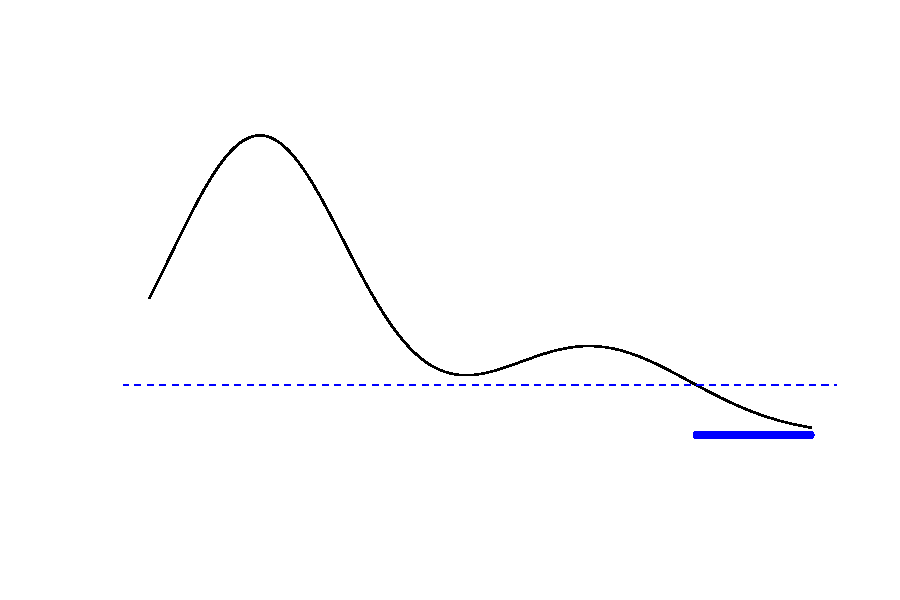
\includegraphics[width=.9\linewidth]{sublevel-set1.pdf}
\end{center}
\end{onlyenv}


\begin{onlyenv}<2>
\begin{center}
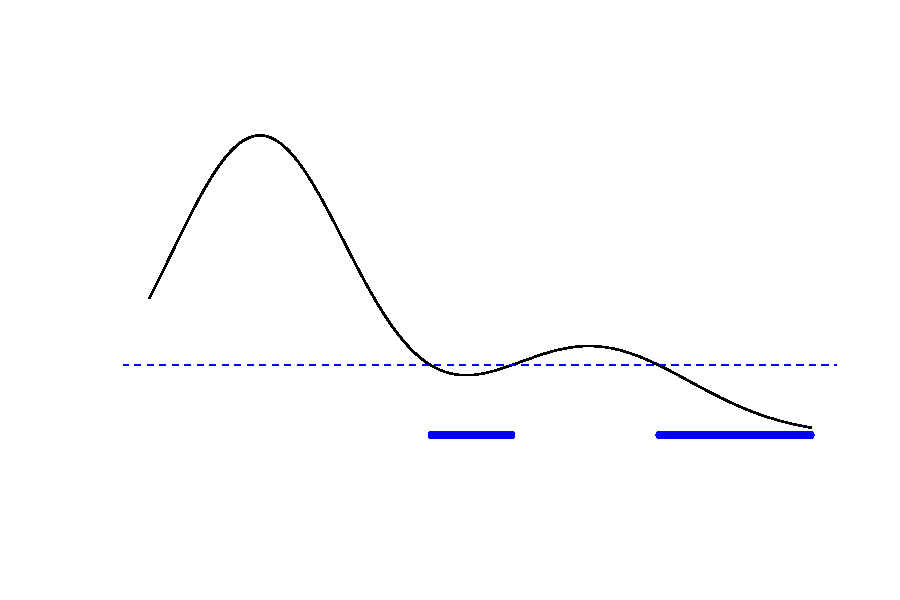
\includegraphics[width=.9\linewidth]{sublevel-set2.pdf}
\end{center}
\end{onlyenv}


\begin{onlyenv}<3>
\begin{center}
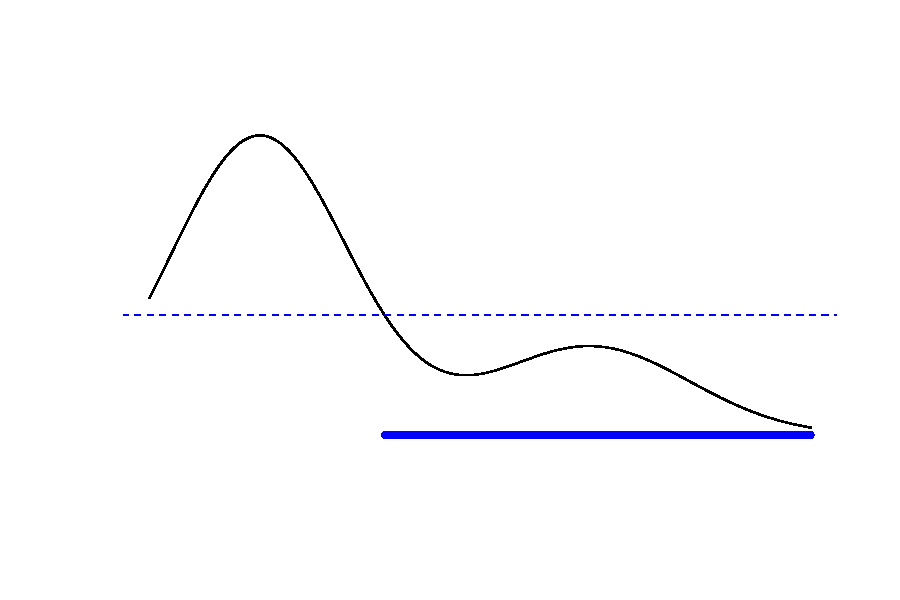
\includegraphics[width=.9\linewidth]{sublevel-set3.pdf}
\end{center}
\end{onlyenv}


\begin{onlyenv}<4>
\begin{center}
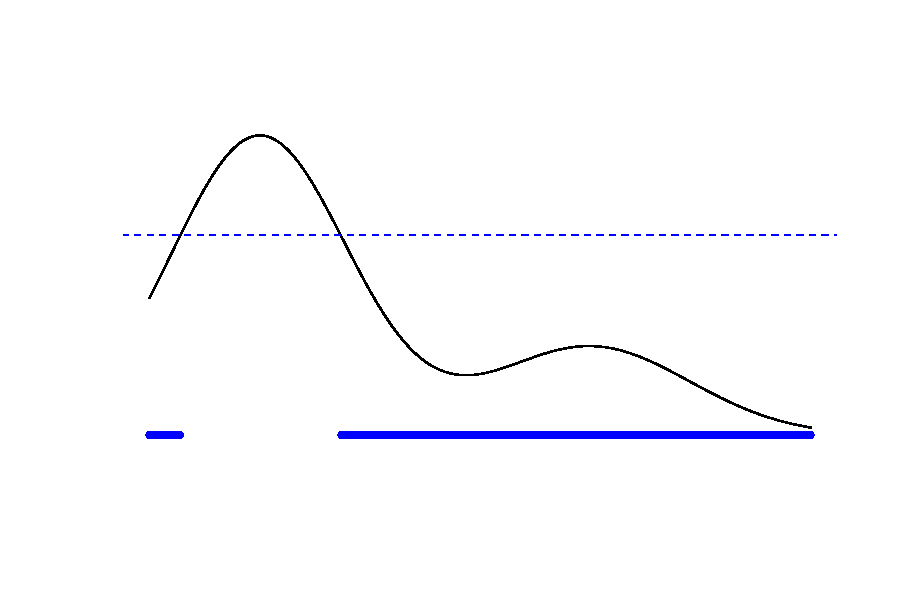
\includegraphics[width=.9\linewidth]{sublevel-set4.pdf}
\end{center}
\end{onlyenv}
\end{frame}



\begin{frame}[label={sec:orgb8e1937}]{Estimand}
We consider the parameter \( \gamma \) defined as the function
\( \gamma(P) \colon [-1,1] \longrightarrow [0,1] \) with
\begin{equation*}
  \gamma(P)(\alpha) =
  P(\mathcal{W}_{\alpha}(P)) =
  P(\tau(P)(W) \leq \alpha).
\end{equation*}

\vfill

Alternative formulation is that $\gamma(P)$ is the cumulative
distribution function of the random variable
\( \tau(P)(W) \in [-1,1] \).

\vfill

Univariate, nondecreasing function which is easy to visualize.

\vfill

\begin{quote} %% 
The value \(\gamma(P)(\alpha)\) is the proportion of the population with an
expected treatment effect below or equal to \(\alpha\). For instance,
\(\gamma(P)(0)\) is the proportion of the population for which the
treatment is not expected to be beneficial.
\end{quote}
\end{frame}


\begin{frame}[label={sec:org78ced7e}]{Illustration of the function \(\gamma(P) \colon [-1,1] \rightarrow [0,1]\)}
\hfill

\begin{onlyenv}<1>
\begin{center}
\texttt{glm(Y $\sim$ age * A + sex)}
\end{center}

\vspace{-1.2cm}

\begin{center}
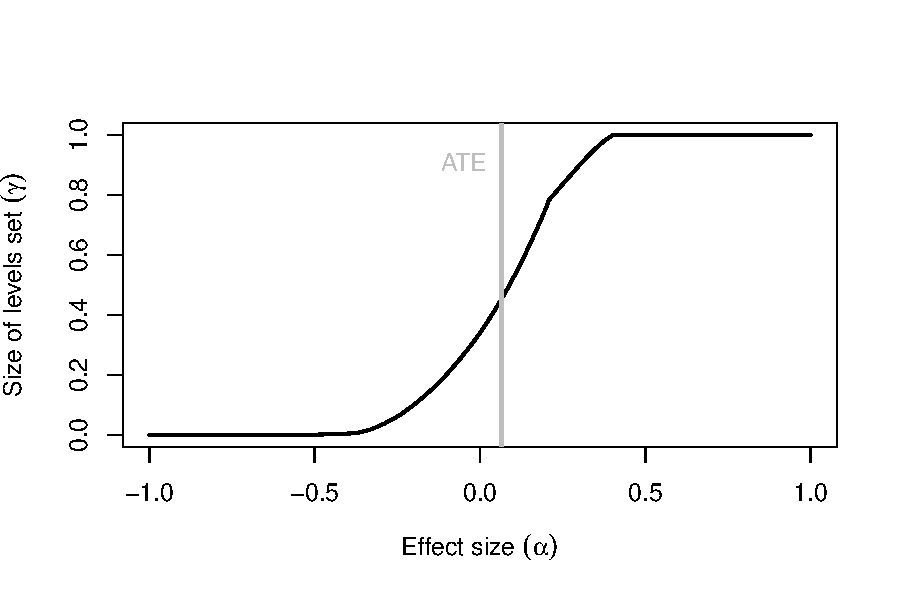
\includegraphics[width=.9\linewidth]{curve-illu-v1.pdf}
\end{center}
\end{onlyenv}

\begin{onlyenv}<2>
\begin{center}
\texttt{glm(Y $\sim$ age * A + sex * A)}
\end{center}

\vspace{-1.2cm}

\begin{center}
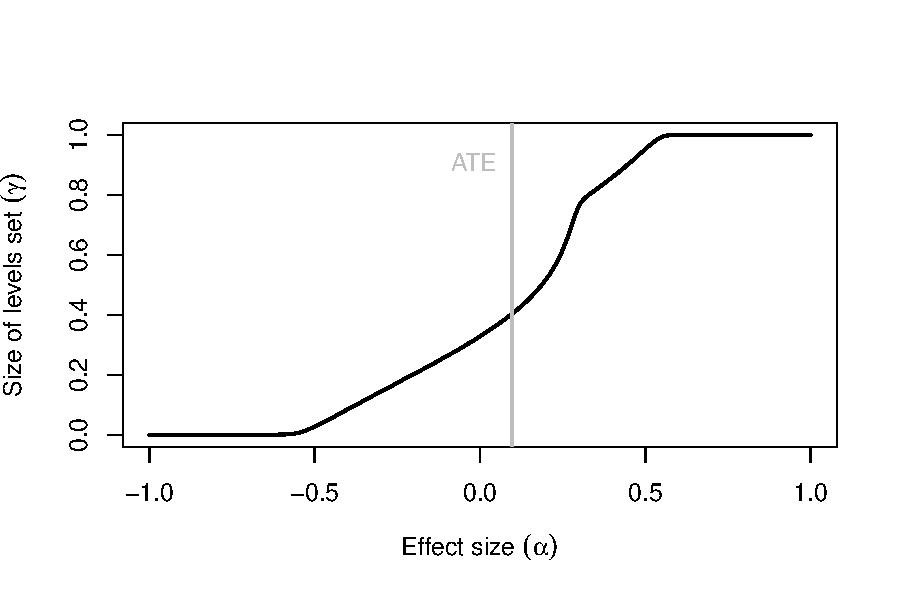
\includegraphics[width=.9\linewidth]{curve-illu-v2.pdf}
\end{center}
\end{onlyenv}

\begin{onlyenv}<3>
\begin{center}
\texttt{glm(Y $\sim$ age + sex + A)}
\end{center}

\vspace{-1.2cm}

\begin{center}
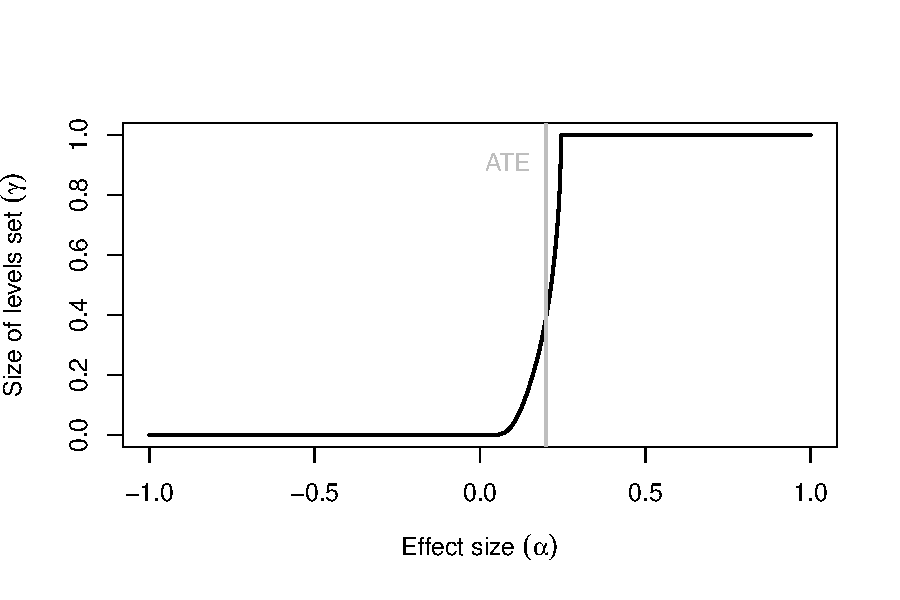
\includegraphics[width=.9\linewidth]{curve-illu-v3.pdf}
\end{center}
\end{onlyenv}

\begin{onlyenv}<4>
\begin{center}
\texttt{glm(Y $\sim$ sex + A)}
\end{center}

\vspace{-1.2cm}

\begin{center}
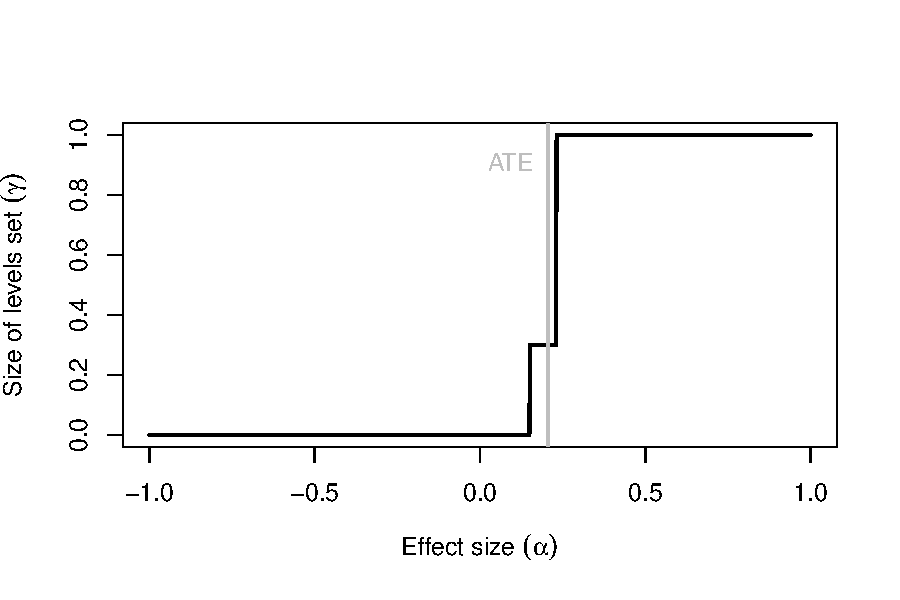
\includegraphics[width=.9\linewidth]{curve-illu-v4.pdf}
\end{center}
\end{onlyenv}
\end{frame}


\begin{frame}[label={sec:org02c4fcb}]{Estimation}
For fixed \(\alpha \in (-1,1)\), the parameter \(P \mapsto
\gamma(P){(\alpha)}\) is not pathwise differentiable (under some
regularity conditions\footnote{Led me to the book ``Differential Topology''
\citep{guillemin2010differential}:
\begin{center}
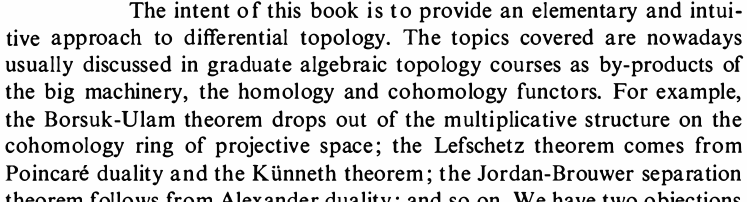
\includegraphics[width=.7\textwidth]{./diff-top-foreword-screenshot.png}
\end{center}}).

\vfill


Necessary condition for the existence of a
regular and asymptotically linear estimator
\citep{van1991differentiable}.

\vfill

\(\implies\) Usual toolbox not available.
\end{frame}



\begin{frame}[label={sec:orgcc66226}]{Estimators}
The standard toolbox is not available \(\rightarrow\) many interesting
procedures to consider:

\vspace{.5cm}


\begin{itemize}
\item ``Naive plug-in'' estimator

\item Generalized Grenander-type estimator

\item Estimate a best approximating spline estimand

\item Orthogonal statistical learning
\end{itemize}

\vfill
\end{frame}


\begin{frame}[label={sec:org246b9ae},fragile]{Naive plug-in (i.e., the obvious) estimator}
 \begin{onlyenv}<1>
\lstset{language=r,label= ,caption= ,captionpos=b,numbers=none}
\begin{lstlisting}
glm_fit <- glm(Y ~ A*Age*Sex, data = sim_dd, family = binomial())

wd0 <- copy(sim_dd)[, A := 0]
wd1 <- copy(sim_dd)[, A := 1]

Y1_hat <- predict(glm_fit, newdata = wd1, type = "response")
Y0_hat <- predict(glm_fit, newdata = wd0, type = "response")
est_cates <- Y1_hat - Y0_hat

Fn <- ecdf(est_cates)
plot(Fn)
\end{lstlisting}
\end{onlyenv}

\begin{onlyenv}<2>
\begin{center}
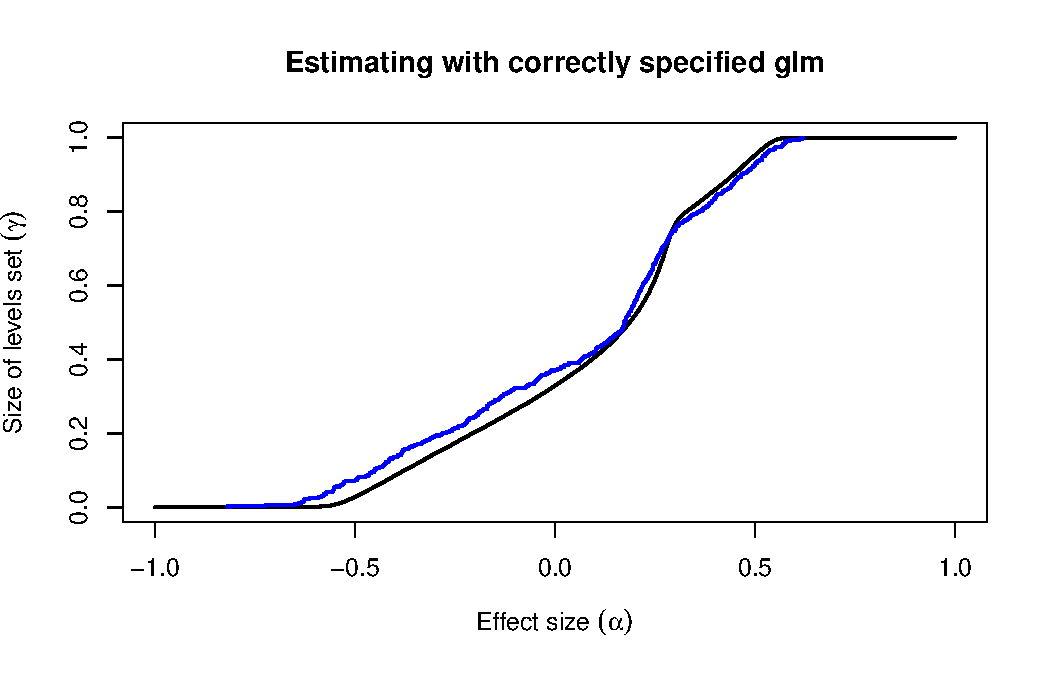
\includegraphics[width=.9\linewidth]{est-gamma-glm1.pdf}
\end{center}
\end{onlyenv}

\begin{onlyenv}<3>
\begin{center}
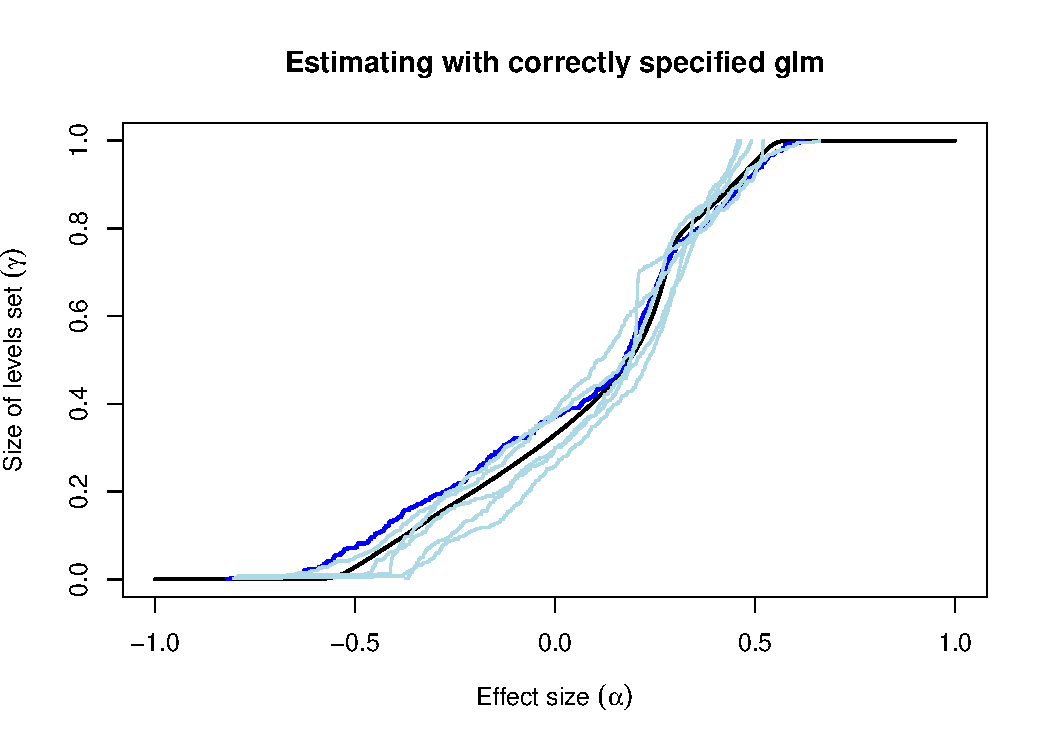
\includegraphics[width=.9\linewidth]{est-gamma-glm2.pdf}
\end{center}
\end{onlyenv}

\begin{onlyenv}<4>
\begin{center}
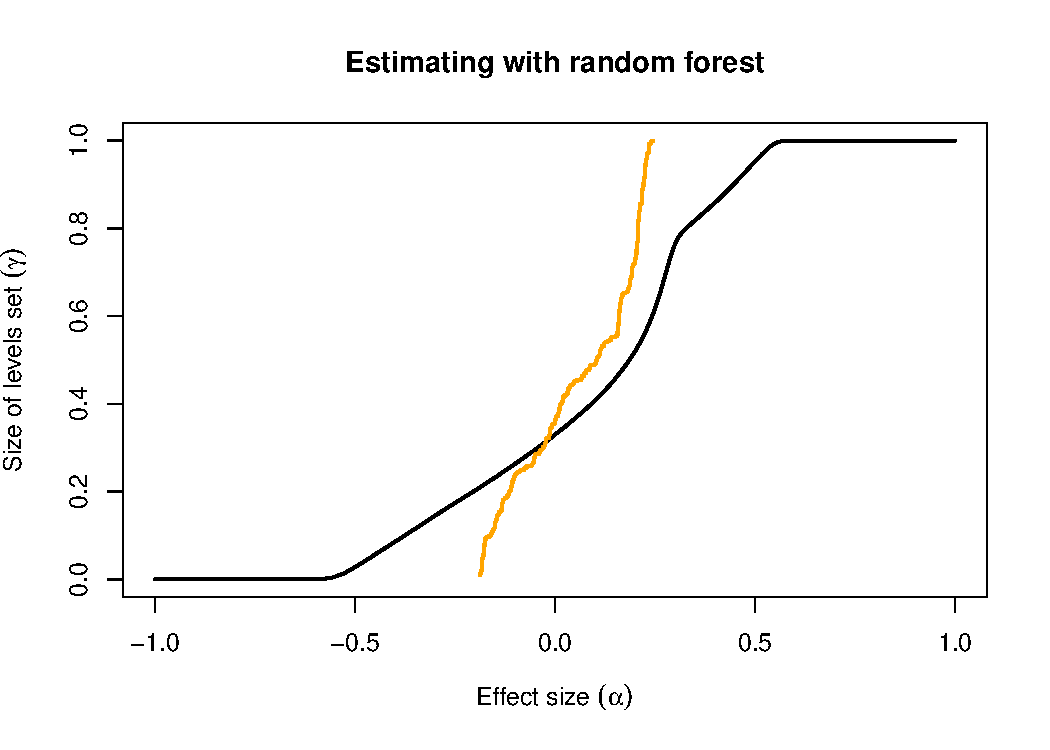
\includegraphics[width=.9\linewidth]{est-gamma-rf1.pdf}
\end{center}
\end{onlyenv}

\begin{onlyenv}<5>
\begin{center}
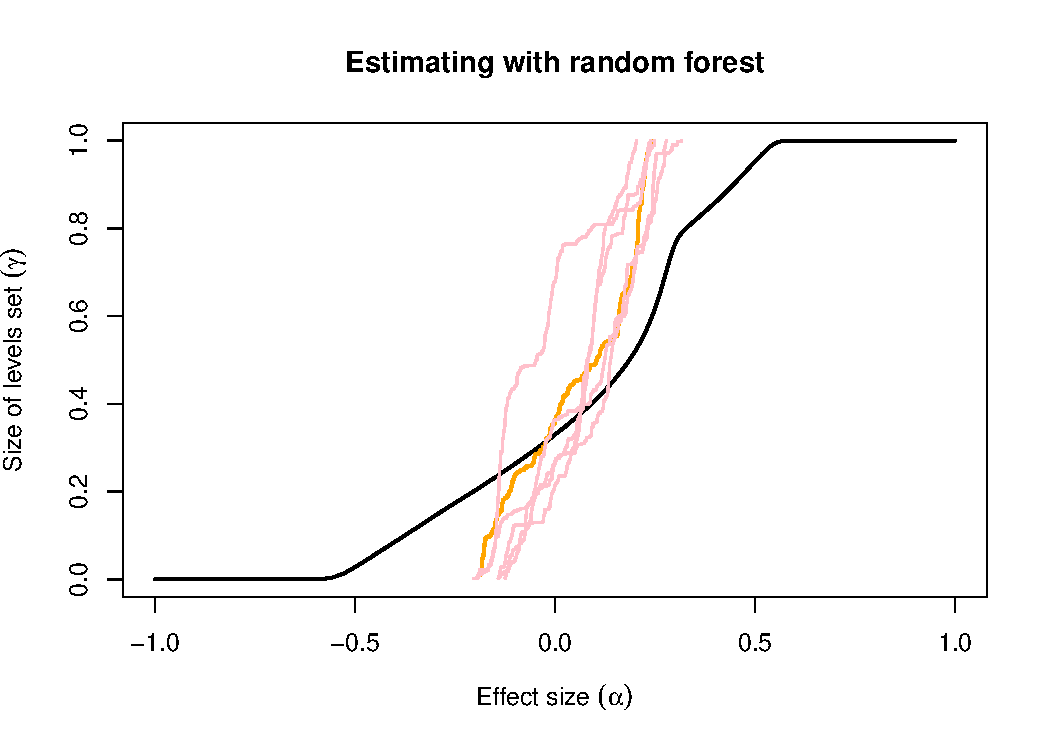
\includegraphics[width=.9\linewidth]{est-gamma-rf2.pdf}
\end{center}
\end{onlyenv}
\end{frame}

\begin{frame}[label={sec:org826d7b7}]{Generalized Grenander-type estimator\footnote{\cite{westling2020unified,van2006estimating,groeneboom1983density,grenander1956theory}}}
The function \(\alpha \mapsto \gamma(P)(\alpha)\) is nondecreasing. The
primitive of a nondecreasing function is convex.

\vfill

\color{bblue}Idea\color{black}:
\begin{enumerate}
\item Estimate the primitive function (aka anti-derivative) \(\alpha \mapsto \Gamma(P)(\alpha) = \int_{-1}^{\alpha} \gamma(P)(u)
   \diff u\)
\item Find the greatest greatest convex minorant of the estimator
\(\hat\Gamma_n\)
\item Estimate \(\gamma\) with the derivative of \(\hat\Gamma_n\)
\end{enumerate}

\vfill

The parameter \(P \mapsto \Gamma(P)(\alpha)\) \emph{is} pathwise
differentiable at points \(\alpha\) at which \(\alpha \mapsto
\gamma(P)(\alpha)\) is continuous.

\vfill

We can use the standard toolbox to estimate \(\Gamma(P)\).
\end{frame}

\begin{frame}[label={sec:org15a37ef}]{Approximate estimand}
\vfill

Estimate an approximation of the function \(\gamma(P)\), e.g., the
best 0- or 1-order spline approximation to \(\gamma(P)\).

\vfill

Splines (with fixed knots) are determined by a set of coefficients.
These coefficient are pathwise differentiable, if the knots are not
placed at points of discontinuity of \(\alpha \mapsto
\gamma(P)(\alpha)\).

\vfill
\end{frame}


\begin{frame}[label={sec:orgbbb6626}]{Orthogonal statistical learning \citep{foster2023orthogonal}}
Extending some of the ideas from the debiased machine learning
literature to more general \emph{statistical learning} -- estimating
function with empirical loss minimization.
\end{frame}

\begin{frame}[label={sec:org0141cdb}]{Challenges}
\vfill

\begin{itemize}
\item Not clear how incorporate the very interesting special case that
\(\alpha \mapsto \gamma(P)(\alpha)\) is the CDF of a Dirac measure =
no heterogeneity.
\end{itemize}

\vfill

\begin{itemize}
\item Inference
\end{itemize}

\vfill
\end{frame}


\begin{frame}[label={sec:orgbca51db}]{Next project}
The function \(\gamma\) can be used to visually investigate if there is
any treatment heterogeneity in the population.

\vfill


But it does not tell us who the people are that respond differently.

\vfill


Approximate the levels sets \(\mathcal{W}_{\alpha}(P)\) with boxes
for suitable choices of \(\alpha\) to identify subgroups that can be
expected to respond differently to treatment.
\end{frame}


\begin{frame}[label={sec:org4201bc7}]{References}
\footnotesize \bibliography{bib.bib}
\end{frame}
\end{document}